\documentclass{beamer}
\usepackage{tikz}
\usepackage{luanumbers}

\LuaNumbersSetup{decimals=1,warnings=error}

\begin{document}
\begin{frame}{Ordinary content}
  Measurement: 3.14159. Integer: 7.
  \begin{itemize}
    \item<1-> First item
    \item<2-> Second value: 2.675
  \end{itemize}
\end{frame}

\begin{frame}{Protected TikZ source}
  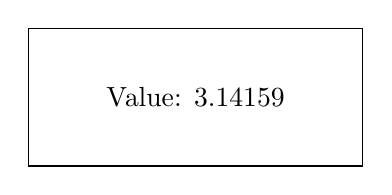
\begin{tikzpicture}[x=1.00cm,y=1.00cm]
    \draw (0.00,0.00) rectangle (4.25,1.75);
    \node at (2.125,0.875) {Value: \LuaNumber{3.14159}};
  \end{tikzpicture}
\end{frame}
\end{document}
